\documentclass[10pt,conference,compsocconf]{IEEEtran}

\usepackage{hyperref}
\usepackage{graphicx}	% For figure environment

% Packages added by Joachim

%drow graph
\usepackage{fancybox}
\usepackage{tikz}
\usepackage{capt-of}
\usepackage{verbatim}

% cancel math expression
\usepackage{cancel}

% math
\usepackage{amsmath}

% url
\usepackage{hyperref}


\begin{document}
\title{PCML CS-433: Higgs Challenge Project}

\author{
  Joachim Muth, SCIPER 214757, joachim.muth@epfl.ch\\
  Junze Bao, SCIPER 266983, junze.bao@epfl.ch\\
  Chanhee Hwang, SCIPER 260872, chanhee.hwang@epfl.ch\\ \\
  \textit{School of Computer and Communication Sciences, EPF Lausanne, Switzerland}
}

\maketitle

%========================
\begin{abstract}
This report presents our work for the first project of PCML course. The project mainly contains two parts: one is to implement six basic model functions and the other is to make predictions for physics particles in a Kaggle competition. With the help of dataset documentation and illustration tables and charts, we found that the train dataset can be separated into eight groups with different number of features. We then applied previously implemented ridge regression and logistic regression model to each group to finally achieve an accuracy of {\color{red} 77\% with ridge regression (TBD)}.
\end{abstract}

%========================
\section{Data description}
The train dataset consists of $N_{tr} = 250000$ events. Each event is associated with an event ID ($int \in [100000, 349999]$), prediction value (our target \textbf{$y_n$} variable) and 30 features (\textbf{$x_n$} feature vector). All 30 features are real valued, except for one feature $PRI\_jet\_num \in \{0, 1, 2, 3\}$ which is categorical. However, some features depend on each other, especially many features are not defined (shown as -999 in the dataset) when the value of the feature jet number is less than or equal to 1. Others, e.g. the last feature $PRI\_jet\_all\_pt$, can be calculated by other features.

The test dataset consists of $N_{te} = 568238$ events ($ID \in [350000, 918237]$). Each event has the same features as the train dataset, with the prediction value being unknown. Therefore our goal is to determine whether an event is a Higgs boson particle event.


%========================
\section{Data preprocessing}

We preprocessed our data and did some feature exploration before selecting a model.

\subsection{Split data}
In order to determine the importance of each feature, and to deal with the great number of \emph{NaN} in the dataset, we first analyzed their distrubutions. 

\cite{higgsChallenge} shows that it is possible to categorize the events into four different groups based on the value of jet number (\emph{int} $\in [0, 3]$), for the fact that some measures are not defined when jet number is a certain value. During the split, we removed the feature jet number for each group because it is always the same value within each group. As mentioned in the data description, the last feature is a sum of all other features. We also removed this feature due to this reason. 

We then obtained four groups with sizes of 99913, 77544, 50379 and 22164 respectively. By skimming through the dataset, we found there are still many undefined values in the first feature $DER\_mass\_MMC$, so we further split each group into two subgroups, one with meaningful mass value $m_H$ and the mass value of the other is \emph{NaN}. Finally we have eight different subgroups.% (see figure \ref{split})

% \begin{figure}[tbp] %-------TIKZ PICTURE---------
%   \centering
% \begin{tikzpicture}[level/.style={sibling distance=20mm/#1}]
% \node [circle,draw] (z){dataset}
%   child {node [circle,draw] (j) {jet = 0}
%   child {node [circle,draw] (l) {$\cancel{m_H}$}
%     child {node [circle,draw] (c){$d, \lambda$}
%       child {node [circle,draw] (p) {ML}
%       }
%     }
%   }
%   child {node [circle,draw] (l) {$m_H$}
%     child {node [circle,draw] (c){$d, \lambda$}
%       child {node [circle,draw] (p) {ML}
%       }
%     }
%   }
% }
%   child {node [circle,draw] (j) {jet = 1}
%   child {node [circle,draw] (l) {$\cancel{m_H}$}
%     child {node [circle,draw] (c){$d, \lambda$}
%       child {node [circle,draw] (p) {ML}
%       }
%     }
%   }
%   child {node [circle,draw] (l) {$m_H$}
%     child {node [circle,draw] (c){$d, \lambda$}
%       child {node [circle,draw] (p) {ML}
%       }
%     }
%   }
% }
%   child {node [circle,draw] (j) {jet = 2}
%   child {node [circle,draw] (l) {$\cancel{m_H}$}
%     child {node [circle,draw] (c){$d, \lambda$}
%       child {node [circle,draw] (p) {ML}
%       }
%     }
%   }
%   child {node [circle,draw] (l) {$m_H$}
%     child {node [circle,draw] (c){$d, \lambda$}
%       child {node [circle,draw] (p) {ML}
%       }
%     }
%   }
% }
%   child {node [circle,draw] (j) {jet = 3}
%   child {node [circle,draw] (l) {$\cancel{m_H}$}
%     child {node [circle,draw] (c){$d, \lambda$}
%       child {node [circle,draw] (p) {ML}
%       }
%     }
%   }
%   child {node [circle,draw] (l) {$m_H$}
%     child {node [circle,draw] (c){$d, \lambda$}
%       child {node [circle,draw] (p) {ML}
%       }
%     }
%   }
% };
% \end{tikzpicture}
%   \caption{Overall view of modelling pipeline. Split the dataset into eight different categories, search 
%   the parameters and calculate the optimal weight.}
%   \vspace{-3mm}
%   \label{split}
% \end{figure}


\subsection{Standardization/Normalization}
In order to work on comparable data, and not to overweight some of them, we apply standardization to raw dataset before any further processes. Normalization, rescaling the raw data down to range $[0, 1]$, is also applied to reduce te complexity of computation so as to avoid potential expoenential overflow when using logsitic regression model.

\subsection{Feature selection}
As our eight groups are well split, we discarded the features only containing \emph{NaN} values. All of the remaining features have meaningful real values, but this does not mean that they are all useful. The histograms of their frequencies show candidates of possibly useless features which have almost no variance. % (see figure \ref{hist})

\subsection{Polynomial building}
Polynomial basis functions can be used to construct more complex and more powerful features, so we constructed a polynomial matrix of degree $d$ with our feature matrix. The degree was chosen by a 4-fold cross validation and is different for each of our 8 groups.

\section{Model selection}

% \subsection{Models descriptions}

% \subsubsection{Least Squares}
% LS resolves the matrix equation between $x^T x \cdot w= x^T y $ to find w. Mathematicaly perfectly correct, its big drawback comes from it high sensitivity to outliers and multicollinear dataset, which is often the case when analysing real-world data.
% \subsubsection{Least Squares Gradient Descent}
% LSGD starts from a initial $w$ matrix and iteratively improves it depending of the gradient $g = \frac{x^T \cdot y-x w}{ \# variables}$. It presents the same weaknesses as LS but provides faster calculation, especially its stochastic variant explained below. 
% \subsubsection{Least Squares Stochastic Gradient Descent}
% Insted of calculating the whole gradient in each iteration as LSGD, LSSGD selects an arbitrary number of small random subsets and calculate the mean between all the their gradient. It's a fast variant of LSGD. The bias  introduced by working with small subsets is compensate by the iterative process.
% \subsubsection{Ridge Regression}
% RR add a regularization term $\lambda$ to the matrix $x^T x$ in order to counter the multicollinearity problem. This $\lambda$ is empirically defined.
% \subsubsection{Logistique Regression}
% LR is based on $\sigma(x) = \frac{e^x}{1 + e^x}$ function which better scales classification problem where $y$'s vector is composed of 
% \subsubsection{Regularized Logistique Regression}



% \begin{table}[htbp]
%   \centering
%   \begin{tabular}[c]{| l | c | c | l | c | c |}
%     \hline
%     Method 	     & te\_loss & accuray \% \\
%     \hline
%     \hline 
%     Least Squares 			& 0.81		& 75.16	    \\
%     Least Squares GD 		& 0.84		& 72.70 	    \\
%     Least Squares SGD 		& 0.83		& 73.54	    \\
%     Ridge Regression 			& 0.82  		& 74.88	\\
%     Logistic Regression		& 666.42  		& 72.14 	\\
%     Regularized Logistic Regr.  	& 666.42  		& 72.14 	\\
% \hline
%   \end{tabular}
%   \caption{Benchmark of six different methods}
%   \label{tab:methods}
% \end{table}



%
%-------------------------
%Least squares: 
%te_loss = 0.81
%accuracy = 0.75
%-------------------------
%Least squares GD: 
%te_loss = 0.84
%accuracy = 0.73
%-------------------------
%Least squares SGD: 
%te_loss = 0.83
%accuracy = 0.74
%-------------------------
%Ridge Regression: 
%te_loss = 0.82
%accuracy = 0.75
%-------------------------
%Logistic Regression: 
%te_loss = 666.42
%accuracy = 0.72
%-------------------------
%Logistic Regression: 
%te_loss = 666.42
%accuracy = 0.72


We only considered ridge regression for linear regression models because optimal $w$ can be derived directly without gradient descent approximation. Ridge regression can also penalize overfitting caused by high polynomial degrees. We also tried logistic regression, which seems to be more suitable for such classification.

\subsection{Ridge Regression}
We applied a 2-steps grid-search method on each of the eight groups for two parameters: polynomial degree $d \in [0, 15]$ and regularization parameter $\lambda \in [1^{-10}, 1]$.  Each pair of parameters is tested through a 4-fold cross-validation and scored by RMSE error. Figure \ref{param} shows the result. Once the best parameters among the intial ranges are chosen for each groups, we narrowed the range and applied again the similar approach to gain more precise parameters. Table \ref{tab:param} sums up the chosen parameters.


\begin{figure}[tbp] %-------TIKZ PICTURE---------
  \centering
  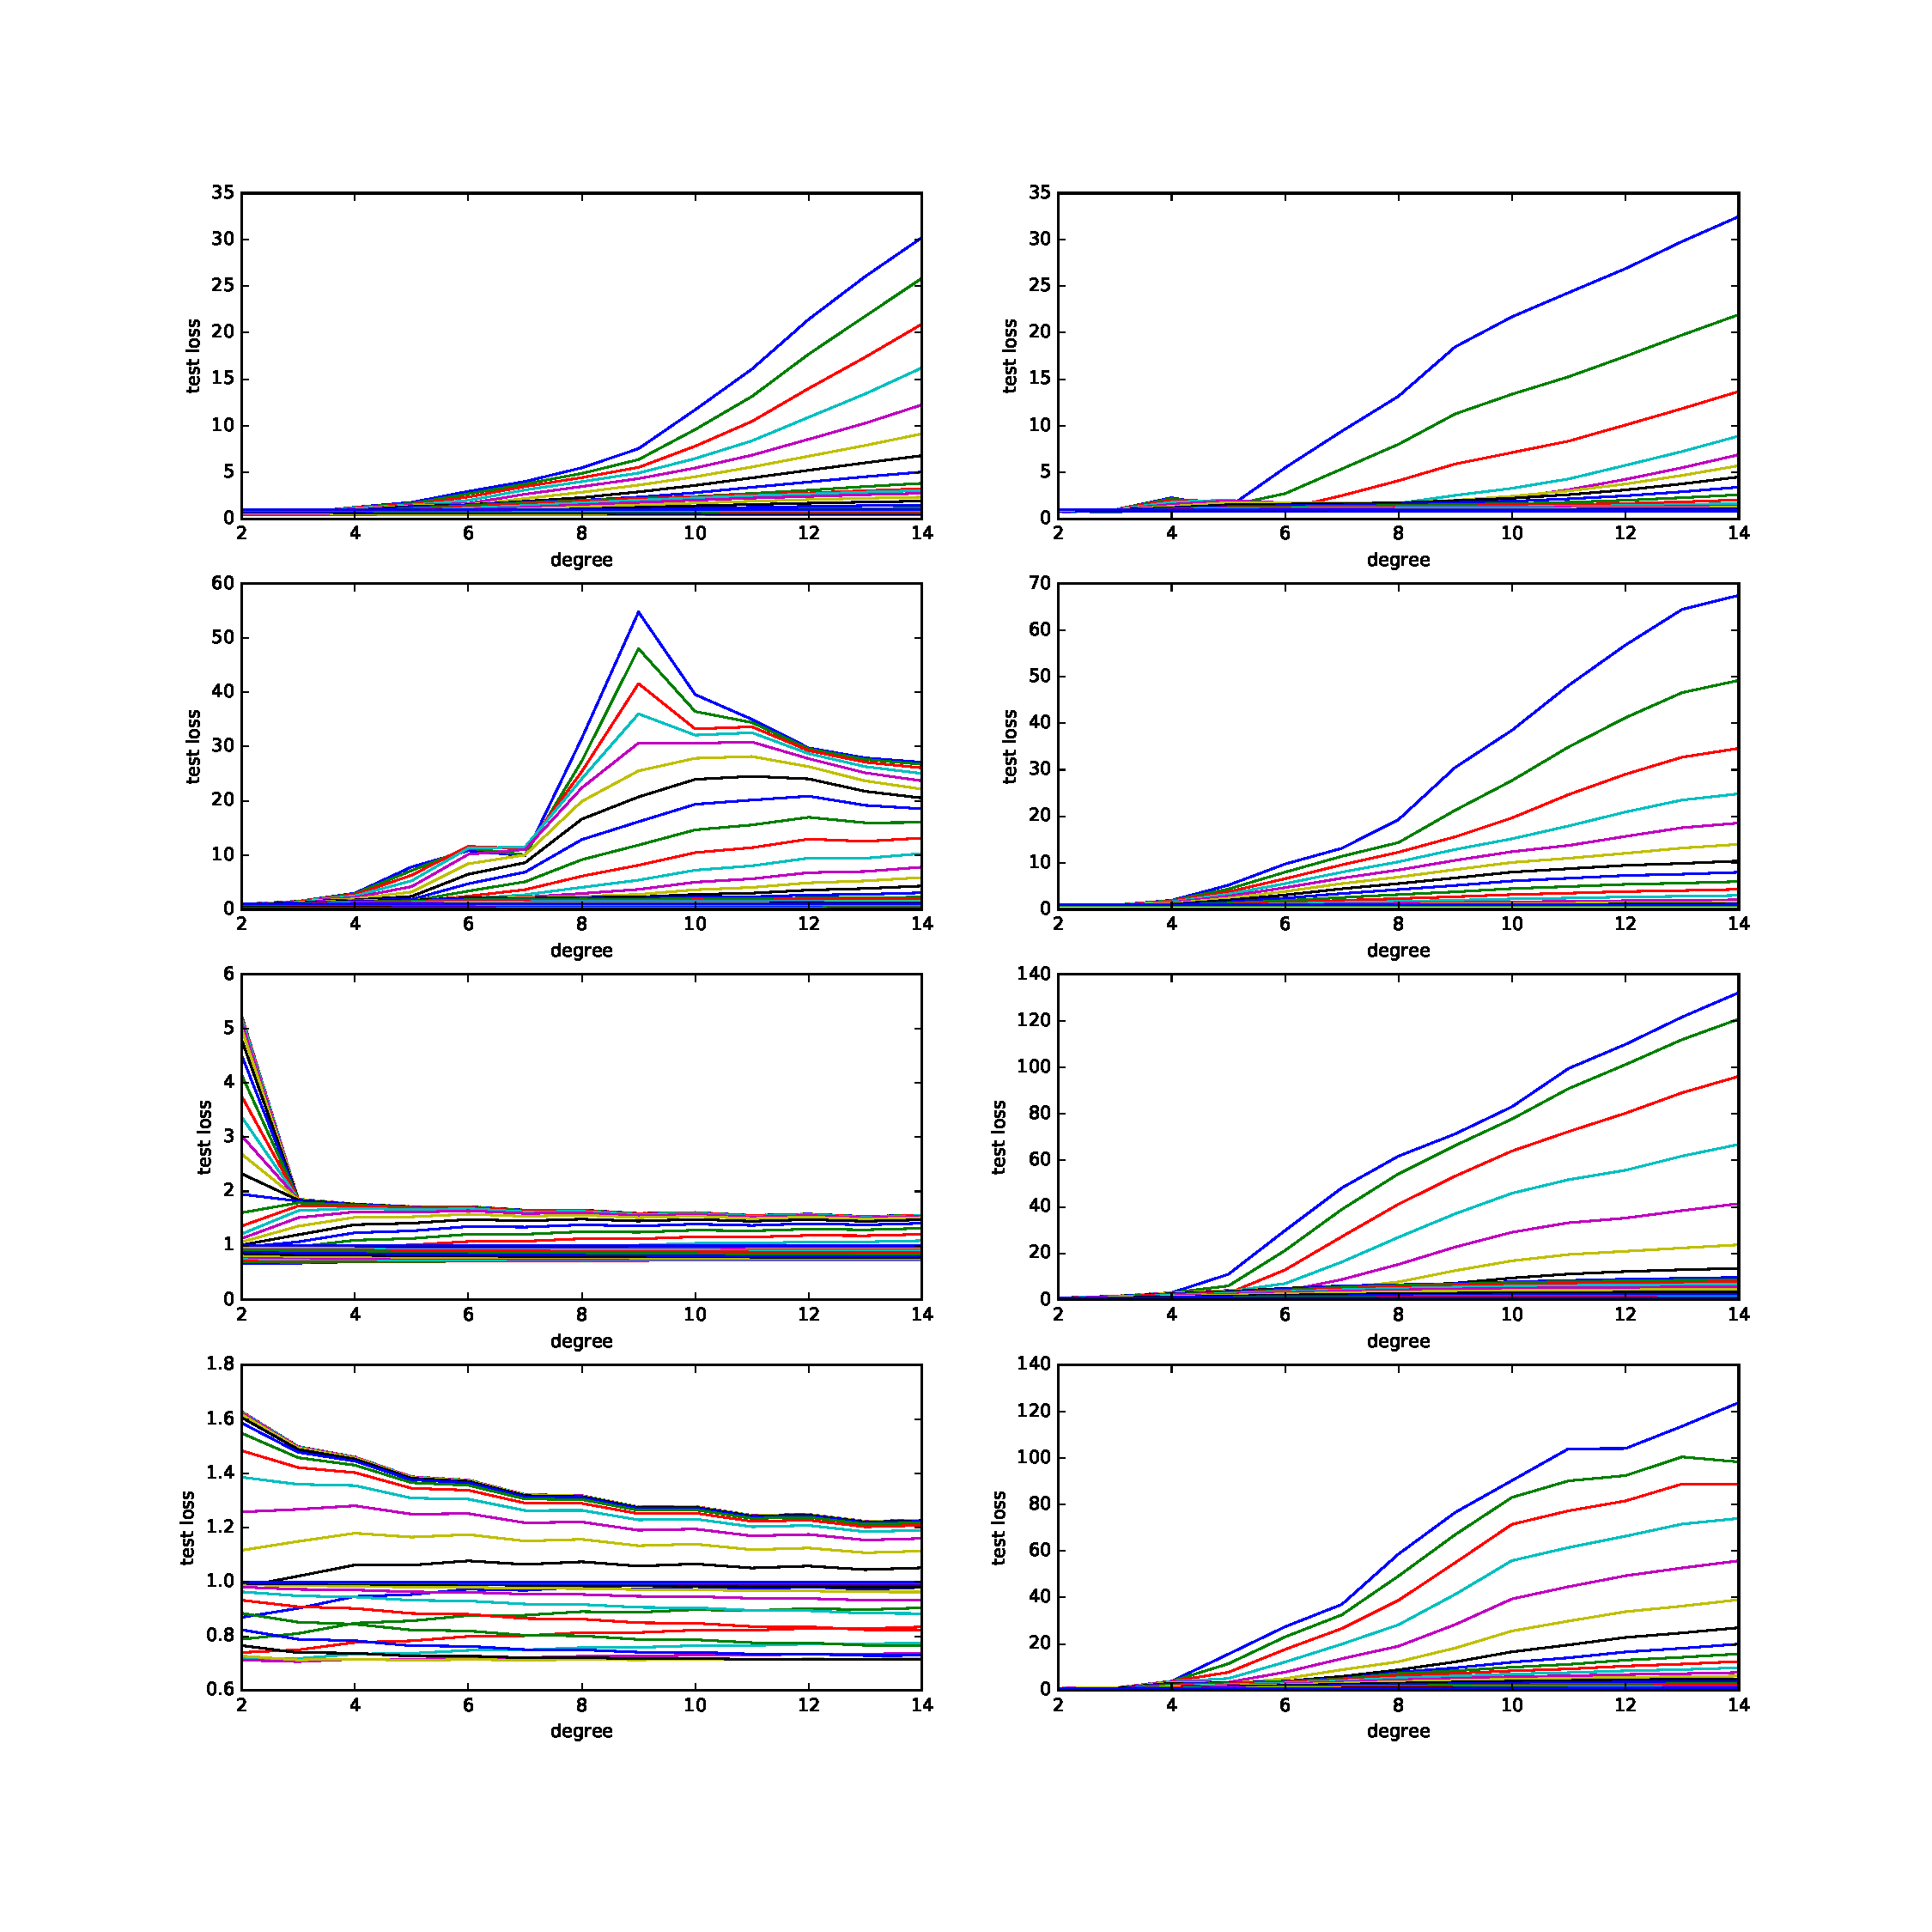
\includegraphics[width=\columnwidth]{img/cross_validation_lot.pdf}
  \caption{Grid search for parameter selection $d$ and $\lambda$ on the eight data subsets. }
  \vspace{-3mm}
  \label{param}
\end{figure}

\subsection{Logistic Regression}
We chose L2-regularized logistic regression for fear of overfitting due to using polynomials. We preset a range of lambdas and degrees, followed by using cross validation to test which pair of parameters produces the best accuracy \footnote{accuracy is calculated as the division of the number of correctly predicted values over the total number of events} for all groups. 

We can still get a real value probablity with logistic regression, although that value will be compared with partition value \footnote{typically the 0.5} when predicting specific class labels. Thus we tried 20 partition values in range $[0.3, 0.8]$, and conclude 0.43 is the best choice for this case because local cross validation accuracy reached the top at that value.

Although we achieved 83\% in local cross validation, eventually we only achieved 76\% in Kaggle with the following parameters: $n_iters = 50000, gamma = 0.000001, lambda_ = 0.01, initial_w = np.zeros(90), cut = 0.43, poly = 2$.

\begin{table}[htbp]
  \centering
  \begin{tabular}[c]{| l | c | c || l | c | c |}
    \hline
    Subset       & lambda & degree & Subset     & lambda      & degree \\
    \hline
    \hline 
    jet0 no mass & 1.599e-05  & 2  & jet0 mass  & 3.237e-05  & 2  \\
    jet1 no mass & 0.1526     & 13 & jet1 mass  & 3.237e-05  & 2  \\
    jet2 no mass & 0.0184     & 2  & jet2 mass  & 7.906e-06  & 3  \\
    jet3 no mass & 0.6250     & 3  & jet3 mass  & 0.0091     & 3  \\
    \hline
  \end{tabular}
  \caption{Selected parameters of Ridge Regression}
  \label{tab:param}
\end{table}

\subsection{Other experiments}
\begin{enumerate}
\item We also tried not to split the dataset into 8 groups, but 4 groups based on jet number or even no groups at all, but expectedly the accuracy did not improve. The (mean) accuracies of no group, 4 groups and 8 groups are 70.19\%, 72.19\% and 80.63\% respectively.
\item When the train dataset is treated as a whole, we thought it would be better to deal with \textit{NaN} values, e.g. replacing $-999$ with the mean or median value of all other events. However unexpectedly the accuracy went down dramatically, e.g. from XXX\% to 71.71\% when replacing with mean value.
\item Another intuition is to increase the polynomial degree to get more complex model, but we noticed when degree is more than {\color{red}XX}, in cross validation the test error increases while the train error decreases, which means overfitting to some extent. We then stop increasing and used the maximum value of degree where the test error and train error are still close. 
\end{enumerate}

%========================
% \section{Results}

% The details of the accuracy of the model over each data subsets are listed on table \ref{tab:details}.

% \begin{table}[htbp]
%   \centering
%   \begin{tabular}[c]{| l| | c | c |}
%     \hline
%     Subset 	& Percentage of Higgs &Accuracy of the model \\
%     \hline \hline
%     jet0 no mass 			& 0.0596		& 0.9437		\\
%     jet0 mass 				& 0.3243		& 0.7866		\\
%     jet1 no mass				& 0.0932		& 0.9067 		\\
%     jet1 mass				& 0.3858	 	& 0.7236 		\\
%     jet2 no mass				& 0.1581		& 0.8699		\\
%     jet2 mass				& 0.5327		& 0.7767		\\
%     jet3 no mass				& 0.0704		& 0.9295		\\
%     jet3 mass				& 0.3203		& 0.7102		\\
%     \hline
%   \end{tabular}
%   \caption{Details of model accuracy}
%   \label{tab:details}
% \end{table}


%========================
% \section{Discussion}



%========================
\section{Summary}
Regularized logistic regression unexpectedly did not give us the best results, while regularized ridge regression works better. Different events have different characteristics, so it is better to separate them based on different features. However, it is tricky to deal with missing values, which has no meaning in physics. Plus, missing value would not be a problem if we separated based on them, which we think should be a better way to deal with missing value.

The model gave us an accuracy of more than $80\%$ when tested by 4-fold cross validation locally. However the accuracy against test dataset only scored $77.748\%$ on Kaggle with ridge regression.


\bibliographystyle{IEEEtran}
\bibliography{literature}

\end{document}
